\section*{Application example}
    Having inputs $U$ and some dated inertial and GNSS measurements $G$, we are able to get a tube enclosing the trailing robot, available on \textsc{Figure}~\ref{fig:trailing}, and a tube enclosing the magnetometer, available on \textsc{Figure}~\ref{fig:magneto}. The estimated angle of the sled according to the trailing vehicle is also showed on the \textsc{Figure}~\ref{fig:phi}.

    \begin{figure}[!htb]
        \begin{subfigure}{0.5\textwidth}
            \centering
            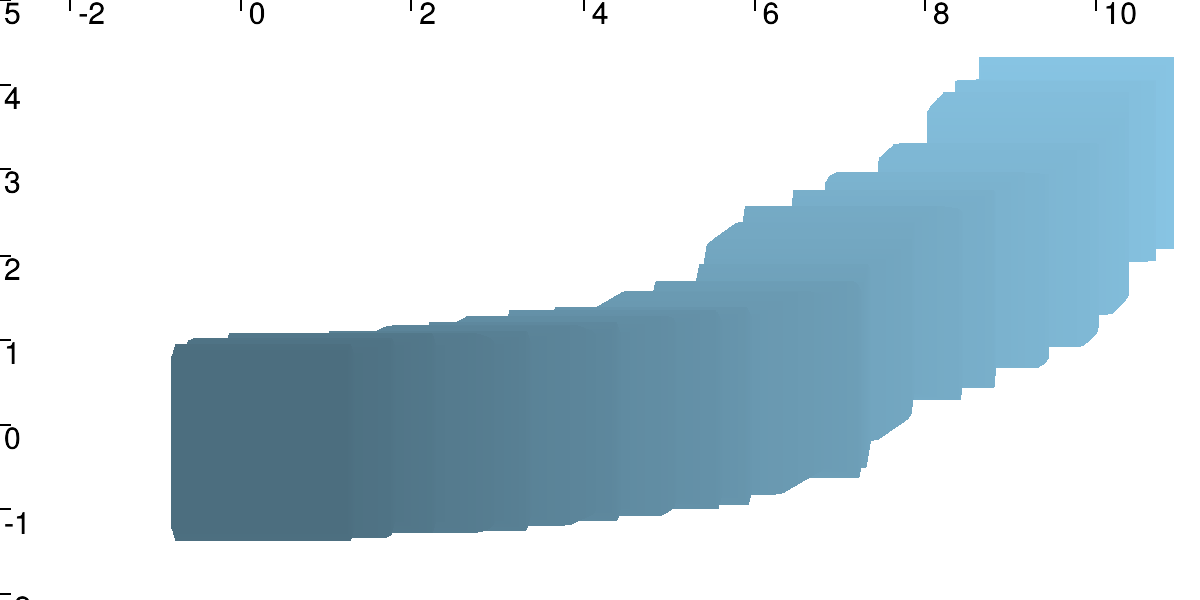
\includegraphics[width=0.8\textwidth]{imgs/example_saturne.png}
            \caption{Trailing robot enclosing tube}
            \label{fig:trailing}
            \hfill
        \end{subfigure}
        \newline
        \begin{subfigure}{0.5\textwidth}
            \centering
            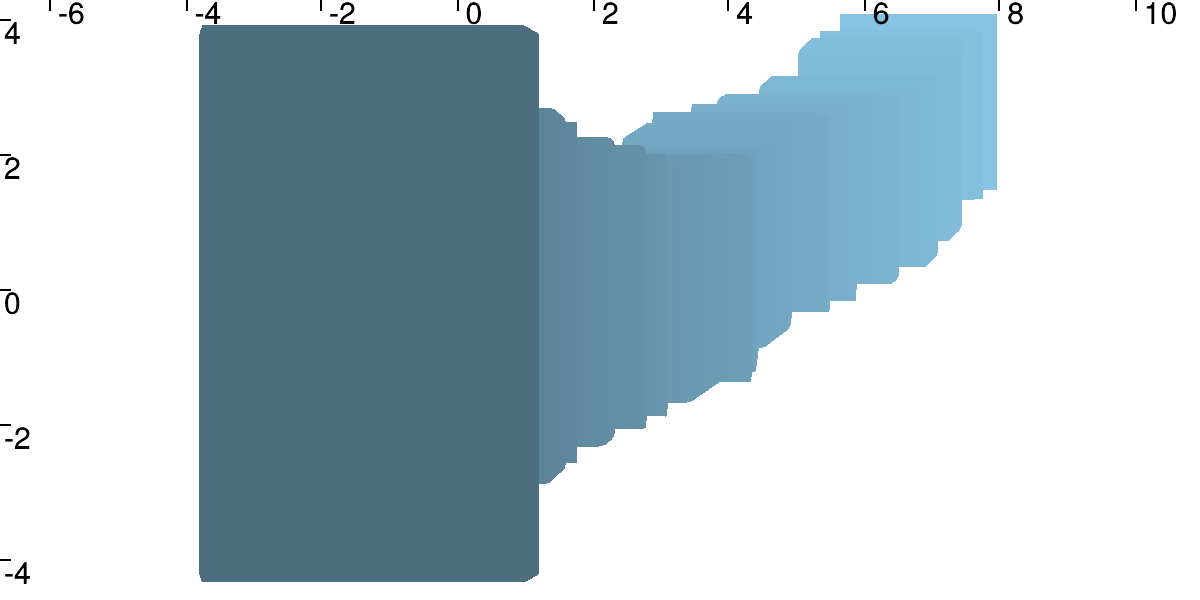
\includegraphics[width=0.8\textwidth]{imgs/example_magnetometer.png}
            \caption{Magnetometer enclosing tube}
            \label{fig:magneto}
            \hfill
        \end{subfigure}
        \newline
        \begin{subfigure}{0.5\textwidth}
            \centering
            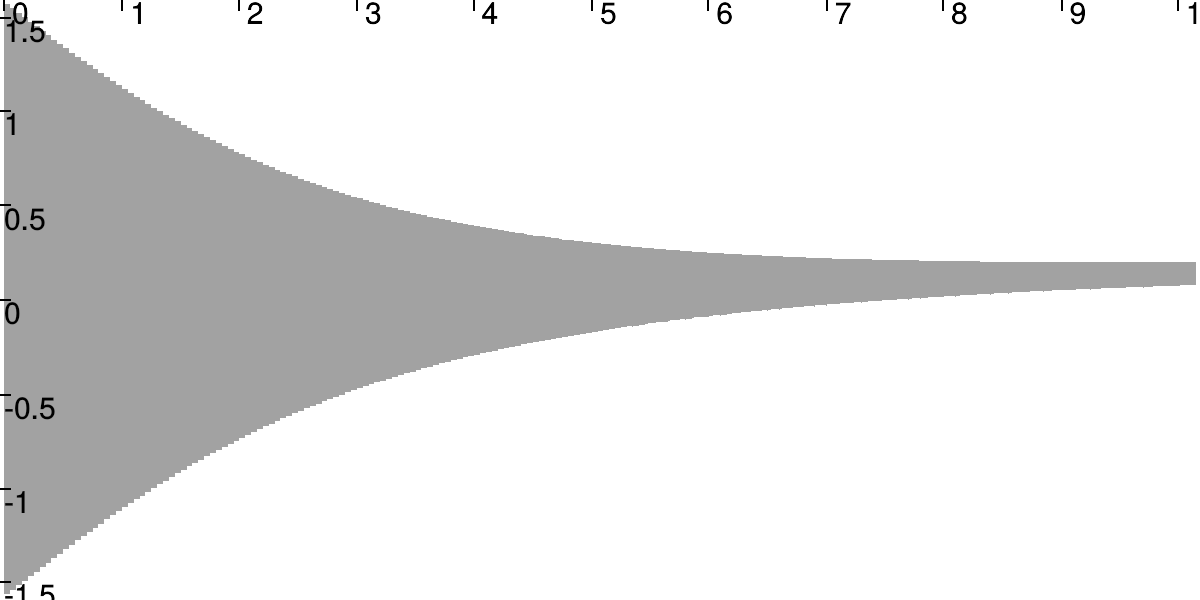
\includegraphics[width=0.8\textwidth]{imgs/example_phi.png}
            \caption{Sled angle estimation}
            \label{fig:phi}
            \hfill
        \end{subfigure}
        \caption{\label{fig:example_tube} Example of enclosing tube}
    \end{figure}
    \hfill

    We could see that the $\phi$ angle is quickly bounded regardless of knowing the initial condition. It let us have a more precise box enclosing the magnetometer. Finally, we are able to have a mapping of the coverage of the magnetometer visible on the \textsc{Figure}~\ref{fig:example_coverage}. Initially the uncertainty on the position of the magnetometer being large, the set of points that can be seen is large and the set of points seen for sure is very small. Then as the robot moves forward, the position of the magnetometer is better known and the set of points seen for sure is increasing.

    \begin{figure}[!htb]
        \centering
        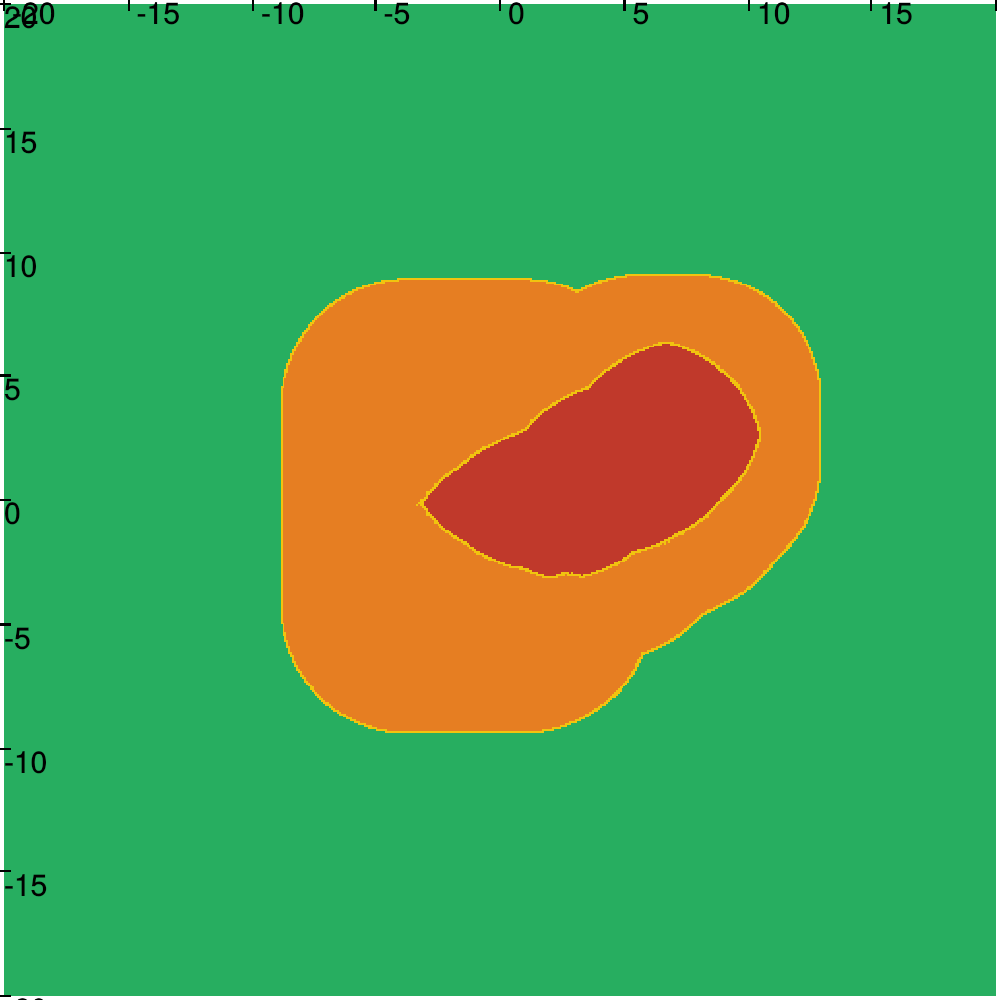
\includegraphics[width=0.4\textwidth]{imgs/example_coverage.png}
        \caption{Mapping coverage}
        \label{fig:example_coverage}
    \end{figure}

